\section{Campo eléctrico}

El campo eléctrico, a diferencia de la fuerza eléctrica, es un concepto abstracto. El concepto de campo eléctrico se basa en la interacción entre cargas ya vista, es decir la Ley de Coulomb, sin embargo no solo da una idea representativa de esta interacción entre cargas, además, permite entender que cada carga individual perturba el espacio a su alrededor, creando así este llamado campo eléctrico.

Suponga que tiene una carga positiva \(q\), y la coloca en un punto dentro de su sistema de referencia inercial, tal y como muestra la figura \ref{fig_ejemplo_campo}. Luego, cerca de la carga, coloca dos placas metálicas cargadas, una positiva y otra negativa. De esta forma, la carga sentirá una fuerza debido a la placa positiva (de repulsión) y una fuerza debido a la placa negativa (de atracción), donde el efecto final será una fuerza como se muestra en la figura.
\begin{figure}[!ht]
  \centering
  \begin{subfigure}[b]{0.45\textwidth}
    \centering
    \begin{tikzpicture}[>=stealth]
      \draw[->,thin] (-.2,0) -- (4,0) node[right] {$x$};
      \draw[->,thin] (0,-.2) -- (0,4) node[left] {$y$};
      \shade[ball color=orange] (2,2) circle (.2) node[above=2mm] {$q$};
    \end{tikzpicture}
    \caption{Carga de prueba.}
  \end{subfigure}
  \hfill
  \begin{subfigure}[b]{0.45\textwidth}
    \centering
    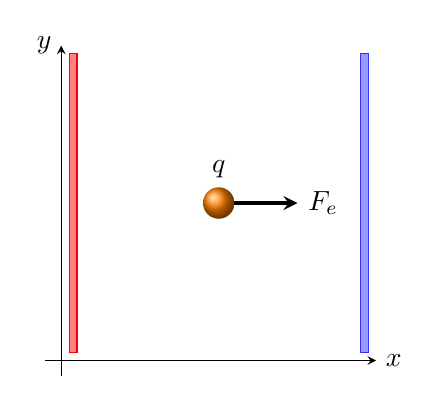
\begin{tikzpicture}[>=stealth]
      \draw[->,thin] (-.2,0) -- (4,0) node[right] {$x$};
      \draw[->,thin] (0,-.2) -- (0,4) node[left] {$y$};
      \draw[very thick,->] (2,2) -- (3,2) node[right] {$F_e$};
      \shade[ball color=orange] (2,2) circle (.2) node[above=2mm] {$q$};
      \draw[red,fill=red!50] (0.1,0.1) rectangle (.2,3.9);
      \draw[blue!80,fill=blue!40] (3.8,0.1) rectangle (3.9,3.9);
    \end{tikzpicture}
    \caption{Campo eléctrico.}
  \end{subfigure}
  \caption{}
  \label{fig_ejemplo_campo}
\end{figure}

Si quitamos esa carga llamada $q$ del lugar, entonces ¿Qué sucede en ese punto que provocaba una fuerza en la carga? Lo que sucede en ese punto es que, en su cercanía, hay dos placas cargadas que influyen en cualquier carga que ahí se coloque. Como las placas metálicas las ha fijado a un lugar específico, entonces no pueden moverse. 

En la figura \ref{fig:concepto_campo_electrico} se muestra un experimento que evidencia este fenómeno entre placas.
\begin{figure}[ht]
  \centering
  \includegraphics[width=0.6\textwidth]{field_concept.jpg}
  \caption{Se visualiza la perturbación del espacio al generar un campo eléctrico como movimiento de cargas.}
  \label{fig:concepto_campo_electrico}
\end{figure}

De esta forma, se puede ver que la fuerza que provocan las placas, en cualquier caso, dependerá de la carga $q$ que se coloque entre ellas. Entonces, conceptualmente, llamamos al efecto generado por las dos placas \emph{campo eléctrico}, que es independiente de la carga (o las cargas) que coloquemos entre ellas. Si bien esta explicación es conceptual, más adelante se profundiza en el calculo de placas cargadas. Para continuar con la deducción del campo eléctrico, tomaremos ejemplos simplificados con cargas puntuales.

\subsection{Deducción del campo eléctrico}

Suponga que tiene una carga positiva y quiere que se quede totalmente quieta. La carga, pues tiene masa, por cuanto siente una fuerza peso provocada por el campo gravitatorio. Entonces, el equilibrio que busca, puede conseguirlo sencillamente. Obtenga alguna carga \( Q \) que a una distancia \( r \) haga que las fuerzas que interactúan con la carga \( q \) se anulen. La figura \ref{fig_campo_g_vs_campo_e} representa esta situación.
\begin{figure}[!ht]
  \centering
  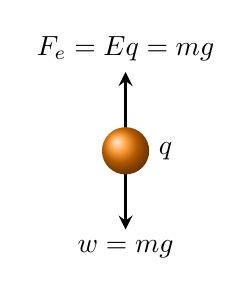
\begin{tikzpicture}[>=stealth]
    \draw[very thick,->] (0,0) -- (0,-1) node[below] {$w=mg$};
    \draw[very thick,->] (0,0) -- (0,1) node[above] {$F_e=Eq=mg$};
    \shade[ball color=orange] (0,0) circle (.3) node[right=3mm] {$q$};
  \end{tikzpicture}
  \caption{Representación de la condición de equilibrio.}
  \label{fig_campo_g_vs_campo_e}
\end{figure}

En definitiva, tendría que encontrar cualquier combinación de \( Q \) y \( r \) que cumpla lo siguiente
\[
  F_g = F_e \rightarrow m\, g - k_e \frac{Q \cdot q}{r^2} = 0
\]

Como las incógnitas son \( Q \) y \( r \), entonces se tienen infinitas soluciones. ¿Qué tienen en común todas las soluciones? 

Todas las soluciones están ocasionando el mismo efecto en \(q\), una fuerza vertical y hacia arriba (en sentido opuesto al peso). Podríamos expresar esto diciendo: 
\begin{quote}
 ``Todas las soluciones generan una perturbación idéntica en el punto del espacio donde se encuentra \(q\)''. 
\end{quote}
 O, en otras palabras, todas las soluciones generan un campo eléctrico de las mismas características en donde está \(q\). Es más, cualquier partícula que coloquemos en el lugar de \(q\), con cualquier carga, por ejemplo una partícula con tres veces la carga $q$ y negativa, sentirá una fuerza proporcional a la que sentía \(q\), pero en sentido opuesto.

En el caso de este ejemplo, \(q\) fué lo que se llama \emph{carga de prueba}, es decir, una carga que se coloca sin importar su valor de carga. Y por otro lado, la carga incógnita \(Q\) fué nuestra carga fuente, aquella que genera un campo eléctrico para causar un efecto sobre cualquier carga \(q\) que se coloque en sus cercanías. Ahora, está listo para definir el campo eléctrico.

\begin{definition}[Campo Eléctrico]
El campo eléctrico \( \vec{E} \) se define como la fuerza por unidad de carga de prueba positiva en un punto en el espacio. Esto puede expresarse como:
\begin{equation}
  \vec{E} = \frac{F}{q^{+}} = k_e \frac{Q}{r^2}
\end{equation}
donde:
\begin{itemize}
  \item \( Q \) es la carga que genera el campo (puntual).
  \item \( r \) es la distancia entre la carga de prueba y \( Q \).
\end{itemize}
\end{definition}

En caso de que exista más de una carga que genera el campo, se aplica el principio de superposición que consiste en sumar todos todos los campos vectorialmente.
\[
  \vec{E} = \sum{\vec{E}_i} = k \cdot \sum{\frac{Q_i}{r^2_i}} \hat{r}_i
\]
\begin{tcolorbox}[myconclusion]
  Cuidado: El campo eléctrico es un campo vectorial, por lo que cuando se suman varios campos, se suman vectorialmente. El resultado de \(\vec{E}\) es la fuerza por unidad de carga que siente una carga \(q^{+}\).
\end{tcolorbox}

Y para el caso particular del ejemplo inicial (figura \ref{fig_ejemplo_campo}), donde se colocan dos placas continuas con carga uniforme, entonces la sumatoria resultará en una integral.

\subsection{Visualización del campo eléctrico}

Como se ha mencionado, la deducción del campo eléctrico se ha realizado usando una carga puntual de prueba \(q\) y una carga puntual fuente \(Q\). Pero en la definición se ha enfatizado que \(\vec{E}\) es una cantidad vectorial. Consecuentemente, visualizar el comportamiento con múltiples cargas y sus interacciones en el campo generado puede ser de gran ayuda complementaria a la explicación anterior.

Como vimos, el campo eléctrico es la fuerza que siente una carga positiva (llamada carga de prueba) cuando se coloca en los alrededores de una carga fuente. Como la carga de prueba es positiva podríamos representar el efecto en diversos puntos para una carga fuente genérica positiva y otra negativa. Al hacer esto vemos que el campo para una carga puntual es siempre radial saliente para cargas positivas y entrante para cargas negativas como se muestra en la figura \ref{fig:campo_electrico}. 

\begin{figure}[ht]
  \centering
  \begin{subfigure}[b]{0.45\textwidth}
    \centering
    \includegraphics[width=\textwidth]{campo_electrico_positivo.png}
  \end{subfigure}
  \begin{subfigure}[b]{0.45\textwidth}
    \centering
    \includegraphics[width=\textwidth]{campo_electrico_negativo.png}
  \end{subfigure}
  \caption{Campo eléctrico de una carga puntual positiva y una negativa.}
  \label{fig:campo_electrico}
\end{figure}

Si se tienen varias cargas eléctricas, el campo eléctrico en un punto es la suma vectorial de los campos generados por cada una de ellas. El efecto gráfico del campo eléctrico puede visualizarse de dos maneras:
\begin{itemize}
  \item Realizar la gráfica de la función vectorial \(\vec{E}\) en el espacio. Esto luce como un mapa de flechas que indican la dirección y magnitud del campo en cada punto.
  \item Realizar las líneas de campo que representan la dirección y magnitud del campo en diversos puntos (se verá con más detalle en la sección \ref{sec:lineas_de_campo}).
\end{itemize}

Siempre recuerde que esta sección se llama electrostática porque las cargas permanecen fijas. La carga de prueba es un concepto matemático para poder encontrar la fuerza en un punto determinado. Y las cargas llamadas fuente son elementos fijos en el sistema de referencia. Así, al colocar la supuesta carga de prueba en un conjunto cuidadosamente seleccionado de puntos (ya que hay infinitos puntos en el plano) puede obtener un diagrama que transmita una idea sobre cómo se comporta el campo eléctrico en cierta región. De esta manera se ha representado un mapa de flechas ilustrativo, que busca dar una idea de como se comporta la fuerza que siente una carga de prueba en una determinada región en la figura \ref{fig:campo_electrico_ejemplo}.
\begin{figure}[ht]
  \centering
  \includegraphics[width=0.5\textwidth]{field_example.png}
  \caption{mapa de la fuerza que siente \(q^{+}\) en cada punto.}
  \label{fig:campo_electrico_ejemplo}
\end{figure}

¿Qué dice este ``mapa de flechas''? Este mapa de flechas representa la fuerza por unidad de carga que genera la carga fuente (las tres cargas en este caso) para una carga de prueba \(q^{+}\) en cada punto. En este caso el mapa está representado en dos dimensiones, si fuese en tres dimensiones sería un mapa de flechas en el espacio tridimensional.

De este resultado se puede concluir que el campo eléctrico se aleja de cargas positivas y se dirige hacia cargas negativas. Además disminuye con el cuadrado de la distancia y es una propiedad del espacio ya no depende de la carga de prueba \( q \), sino solo de las cargas fuente colocadas \( Q_i \).

Es muy importante tener en cuenta las premisas usadas para formular el campo eléctrico:
\begin{itemize}
  \item \textit{La carga fuente modifica el espacio circundante:} El campo eléctrico es una propiedad del espacio y es generado por una carga fuente.
  \item \textit{El campo es independiente de la carga de prueba:} La carga de prueba se usa solo como herramienta de medición.
  \item \textit{El campo es un campo vectorial:} Tiene dirección y magnitud en cada punto del espacio.
  \item \textit{El campo sigue el principio de superposición:} Si hay varias cargas, el campo total en un punto es la suma vectorial de los campos generados por cada una.
  \item \textit{La carga de prueba es positiva:} Para determinar el sentido del campo es importante tener en cuenta que la carga de prueba es positiva, esto permite ver con claridad cuando el campo es entrante o saliente para una carga puntual, o poder predecir correctamente el sentido del campo en una distribución de cargas (ya sea discreta o continua).
\end{itemize}

\subsection{Distribución continua de campo eléctrico}

Tal y como se presentó la ley de Coulomb y el campo eléctrico, no son de gran utilidad. Esta afirmación se debe a que en la vida real, rara vez encontraremos una carga puntual aislada. 

Frecuentemente, en física, el concepto de partícula, corpúsculo y de carga puntual son casos extremadamente idealizados, pero simples, que permiten deducir los comportamientos ignorando factores como el tamaño de los cuerpos, la distribución de su masa, distribución de carga o su forma particular. Lo que los transforma en elementos ideales para conformar luego cuerpos más grandes que se acercan más a objetos reales. A estos objetos más grandes conformados por partículas idealizadas les denominaremos cuerpos, y su comportamiento estará dado por la suma de todas las pequeñas interacciones que ocurran en las cargas que lo conforman. Adicionalmente diremos que estos cuerpos son continuos, o en otras palabras, podremos integrar usando las leyes que rigen a los pequeños corpúsculos que lo conforman.

\begin{tcolorbox}[myconclusion]
  Un cuerpo es una distribución continua de partículas, ya sea masa, carga o lo que se quiera analizar. Esto implica que el cuerpo no es discreto, es decir, no puede analizarse como la simple suma de todos sus comportamientos, ya que el cuerpo tiene infinitos corpúsculos que lo conforman. Esto implica necesariamente que debemos realizar una integral, que no es más que la suma de los infinitos comportamientos de cada corpúsculo infinitesimal.
\end{tcolorbox}

\begin{definition}[Distribución continua]
Se denomina una distribución continua de campo eléctrico a un cuerpo cargado, que no es otra cosa más, que un objeto formado por cargas eléctricas que forman un campo eléctrico a su alrededor. Matemáticamente y geométricamente hablando se pueden distinguir tres tipos de distribuciones continuas: lineales, superficiales y volumétricas.
\end{definition}

La distribución lineal de carga, representa un cable. Pues este cable también resulta ideal, ya que no tiene superficie ni volumen, sin embargo es una buena aproximación a un hilo delgado. La distribución superficial representa un plano, la cascara de una esfera, o una superficie cualquiera. Sin embargo al igual que con la distribución lineal, es una superficie ideal, mas no tiene grosor. Por último la distribución volumétrica representa un objeto tridimensional, como por ejemplo un toroide macizo, una esfera maciza o cualquier forma que tenga alto, ancho y espesor. Este tipo de cuerpos también son ideales ya que no presentan rugosidad y la carga se supone uniforme.

Habiendo distinguido los tres tipos de cuerpos, entonces puede enunciar la ecuación del campo eléctrico en un punto para una distribución de carga lineal.
\[
\vec{E} = k \lim_{\Delta q_i \to 0} \sum_i{\frac{\Delta q_i}{r_i^2}\hat{r}_i} = k \int \frac{dq}{r^2} \hat{r}
\]

Si bien esta integral teórica puede resultar terrorífica a primera vista, es generalmente sencilla de resolver para curvas conocidas. Un detalle importante es que cuando se calcula el campo eléctrico producido por esta distribución de carga en un punto, es necesario saber la \emph{densidad de carga}. Tal vez se pregunte ¿Qué es la densidad de carga?

La densidad de carga es una \emph{medida de cuánta carga eléctrica hay distribuida} sobre una determinada región del espacio. Se utiliza cuando las cargas no están concentradas en puntos, sino distribuidas sobre líneas, superficies o volúmenes. Justamente, aplicable a los cuerpos que ha visto anteriormente. Dependiendo del tipo de distribución, hay tres formas principales:

\paragraph{1. Densidad lineal de carga:}

Se usa cuando la carga está distribuida a lo largo de una línea (como un alambre).
\[
  \lambda = \frac{Q}{\ell} \quad \Rightarrow \quad dq = \lambda d\ell
\]
\begin{itemize}
  \item \( \lambda \): densidad lineal, medida en Coulomb por metro (\unit{\coulomb\per\meter}),
  \item \( Q \): cantidad de carga por unidad de longitud,
  \item \( \ell \): longitud del alambre.
\end{itemize}

De esta manera, un alambre fino (ideal), puede ser considerado como un cuerpo de distribución lineal, cuya densidad lineal de carga \(\lambda\) es un determinado valor. Si, a modo de ejemplo, tiene un cable con una densidad lineal de carga \(\lambda = \qty{6}{\micro\coulomb\per\meter}\), significa que por cada metro de cable, hay \qty{6}{\micro\coulomb} de carga distribuidos infinitesimalmente.

Por otro lado, la fracción \(Q/\ell\) establece una relación entre la densidad lineal de carga y el cuerpo con sus dimensiones reales. Así, por ejemplo, para el cable con \(\lambda = \qty{6}{\micro\coulomb\per\meter}\), si el cable tiene una longitud \(\ell=\qty{3}{\metre}\), significa que 
\begin{gather*}
  \lambda = \qty{6}{\micro\coulomb\per\meter} = \frac{Q}{\qty{3}{\metre}} \\ 
  \therefore \quad Q = \qty{6}{\micro\coulomb\per\meter}\cdot\qty{3}{\metre} = \qty{18}{\micro\coulomb}
\end{gather*}
Donde los \qty{18}{\micro\coulomb} están distribuidos de forma continua a lo largo de los \qty{3}{\metre} de longitud del cable.

\paragraph{2. Densidad superficial de carga:}

Se usa para cargas sobre una superficie (como una lámina metálica cargada).
\[
  \sigma = \frac{Q}{A} \quad \Rightarrow \quad dq = \sigma dA
\]
\begin{itemize}
  \item \( \sigma \): densidad superficial, medida en Coulomb por metro cuadrado (\unit{\coulomb\per\meter\squared}),
  \item \( Q \): carga sobre unidad de área,
  \item \( A \): área considerada.
\end{itemize}

Aquí el concepto de distribución superficial de carga es análogo al de distribución lineal, solo que aplicado a una superficie. En otras palabras, \(\sigma\) representa la cantidad de carga distribuida infinitesimalmente en una unidad de superficie.

\paragraph{3. Densidad volumétrica de carga:}

Se usa cuando la carga ocupa un volumen (como una nube de plasma).
\[
  \rho = \frac{Q}{V} \quad \Rightarrow \quad dq = \rho dV
\]
\begin{itemize}
  \item \( \rho \): densidad volumétrica, medido en Coulomb por metro cúbico (\unit{\coulomb\per\cubic\meter}),
  \item \( Q \): carga dentro de una unidad de volumen,
  \item \( V \): volumen correspondiente.
\end{itemize}

Este caso también es análogo a los dos anteriores, pero aplicado a un volumen.

Para concluir sobre el razonamiento detrás de la idea de cuerpo continuo y su densidad de carga, se presenta un ejemplo.

\begin{example}
  Calcular la fuerza que ejerce una varilla de longitud \(\ell\), cargada con una densidad lineal de carga \(\lambda\), sobre una partícula cargada \(Q\) situada en la misma línea de la varilla a una distancia \(a\) de su extremo. La figura \ref{fig_cargas_barra_consigna} representa un esquema del enunciado.
  \begin{figure}[!ht]
    \centering
    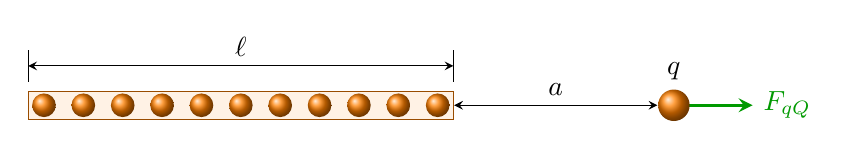
\begin{tikzpicture}[>=stealth]
      \draw[very thick,green!60!black,->] (0,0) -- (1,0) node[right] {$F_{qQ}$};
      \shade[ball color=orange] (0,0) circle (.2) node[above=2mm] {$q$};
      \draw[thin,color=orange!60!black,fill=orange!10] (-2.8,-.18) rectangle (-8.2,.18);
      \foreach \x in {3,3.5,4,...,8} {
        \shade[ball color=orange] (-\x,0) circle (.15);
      }
      \draw[thin,<->] (-.21,0) -- node[above] {$a$} (-2.79,0);
      \draw[thin] (-2.8,.3) -- (-2.8,.7);
      \draw[thin] (-8.2,.3) -- (-8.2,.7);
      \draw[thin,<->] (-2.8,.5) -- node[above] {$\ell$} (-8.2,.5);
    \end{tikzpicture}
    \caption{}
    \label{fig_cargas_barra_consigna}
  \end{figure}

  \textit{Solución}: La varilla tiene una densidad de carga \(\lambda\), de modo tal que la carga total es \(Q=\lambda \ell\). A partir de la ley de Coulomb, 
  \[
    \vec{F}_{12}=k_e \frac{q_1 q_2}{r^2}\hat{r}
  \]
  puede plantear las distancias de una porción pequeña de varilla \(d\ell\) a la carga \(q\). A cada \(d\ell\) le corresponderá una cantidad de carga \(dQ\) dada por la carga misma de la varilla. Como la densidad de carga es lineal y su valor es \(\lambda\) puede escribir la fuerza entre \(dQ\) y \(q\) como 
  \[
    F=k_e\frac{dQ \, q}{r^2} \quad \text{y} \quad dQ=\lambda d\ell
  \]
  de modo que puede escribirse la fuerza en términos de \(\lambda\),
  \begin{equation}\label{eq_ej_fuerza_varilla}
    F=k_e \frac{\lambda d\ell \, q}{r^2}
  \end{equation}
  Ahora, basta con encontrar una forma de representar la distancia \(r\). Se sabe que \(r\) depende de \(\ell\), pero \(r\) representa la distancia de cada \(dQ\) a \(q\). Haga lo siguiente: coloque un sistema de referencia con origen en \(q\), de modo que resulte tal y como se observa en la figura \ref{fig_cargas_barra_sistema_de_referencia}.
  \begin{figure}[!ht]
    \centering
    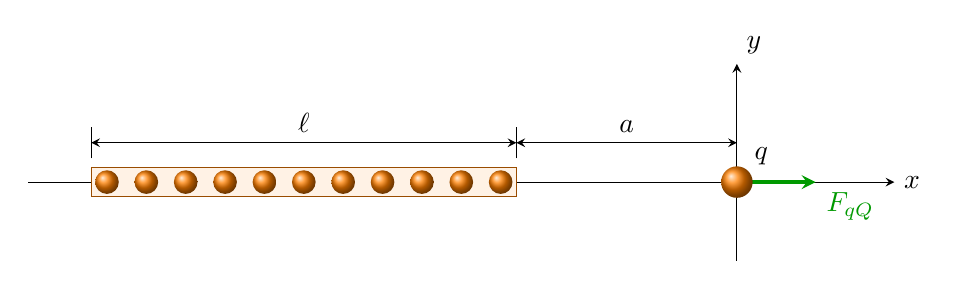
\begin{tikzpicture}[>=stealth]
      \draw[thin,->] (-9,0) -- (2,0) node[right] {$x$};
      \draw[thin,->] (0,-1) -- (0,1.5) node[above right] {$y$};
      \draw[very thick,green!60!black,->] (0,0) -- (1,0) node[below right] {$F_{qQ}$};
      \shade[ball color=orange] (0,0) circle (.2) node[above right=1mm] {$q$};
      \draw[thin,color=orange!60!black,fill=orange!10] (-2.8,-.18) rectangle (-8.2,.18);
      \foreach \x in {3,3.5,4,...,8} {
        \shade[ball color=orange] (-\x,0) circle (.15);
      }
      \draw[thin,<->] (0,.5) -- node[above] {$a$} (-2.8,.5);
      \draw[thin] (-2.8,.3) -- (-2.8,.7);
      \draw[thin] (-8.2,.3) -- (-8.2,.7);
      \draw[thin,<->] (-2.8,.5) -- node[above] {$\ell$} (-8.2,.5);
    \end{tikzpicture}
    \caption{}
    \label{fig_cargas_barra_sistema_de_referencia}
  \end{figure}

  Ahora, una distancia arbitraria \(x\) sobre la barra será 
  \[
    r=a+x \quad \text{con } x<a ~ \text{y} ~ x>\ell
  \]
  Reemplazando esta última expresión en la ecuación \eqref{eq_ej_fuerza_varilla}, resulta 
  \[
    F=k_e \frac{\lambda d\ell \, q}{(x+a)^2}
  \]
  Pero como la variable de longitud que se ha elegido es \(x\), entonces un \(d\ell=dx\), de modo que se puede sustituir en la expresión final, 
  \[
    F=k_e \frac{\lambda dx\, q}{(x+a)^2}
  \]
  Como se quiere sumar cada pequeña contribución de cada porción de carga de la varilla, entonces integramos respecto de \(x\),
  \begin{gather*}
    F_{qQ}=\int_{\ell+a}^a k_e\frac{\lambda dx \, q}{(x+a)^2} \\ 
    F_{qQ}=k_e q \lambda \int_{\ell+a}^a \frac{1}{(x+a)^2}dx
  \end{gather*}
  Esta integral puede resolverse por sustitución, donde el resultado es 
  \begin{gather*}
    F_{qQ} = k_e q \lambda \left( -\frac{1}{2a}+\frac{1}{\ell+2a} \right) \\ 
    F_{qQ} = -k_e\frac{\ell \lambda q}{2a(\ell+2a)}
  \end{gather*}
  Como se ha realizado el cálculo empleando el lado negativo del eje de abscisas, entonces la última expresión espera valores de \(\ell\) negativos. En general, esta expresión se presentará para colocar valores de \(\ell\) positivos (ya que en general una distancia no se considera negativa). De esta manera, puede alternar el signo resultante para obtener la expresión final, donde
  \[
    \boxed{F_{qQ} = k_e\frac{\ell \lambda q}{2a(\ell+2a)}}
  \]
  no presenta signo negativo, ya que \(\ell\) será positivo.
\end{example}
